\documentclass[runningheads]{llncs}

\usepackage[T1]{fontenc}
\usepackage{graphicx}
\usepackage{amsmath}
\usepackage{amssymb}
\usepackage{booktabs}
\usepackage{array}
\usepackage{microtype}
\usepackage[hidelinks]{hyperref}
\renewcommand\UrlFont{\rmfamily}

\graphicspath{{figures/}}
\renewcommand{\topfraction}{0.9}
\renewcommand{\textfraction}{0.1}
\renewcommand{\floatpagefraction}{0.8}

\begin{document}

\title{ProtoHedge Beyond Simulation: Real-Market Performance and Explanations of Interpretable Deep Hedging}
\titlerunning{ProtoHedge Beyond Simulation}

\author{Yanis Zaim\inst{1} \and Sayak Chakrabarty\inst{2} \and Imon Banerjee\inst{2}}
\authorrunning{Y. Zaim et al.}
\institute{Columbia University, New York, NY, USA\\
\email{ymz2108@columbia.edu} \and
Northwestern University, Evanston, IL, USA\\
\email{\{sayak.chakrabarty,imon.banerjee\}@northwestern.edu}}

\maketitle

\begin{abstract}
ProtoHedge chooses each hedge by consulting a small collection of dated market states, its prototypes,
and so can cite the past situations behind a decision. It was evaluated only in simulation. We test it on
twenty years of US option data for ten underlyings: the liabilities are synthetic European and Asian calls,
and the hedges trade the underlying and a listed call at historical prices and quotes. We ask how much
hedging performance the interpretable model retains, and when a reader can trust the past state it cites.
The released model reduces the standard deviation of the hedging error by 88.5\% (European) and 84.9\%
(Asian), against 93.3\% and 88.7\% for Deep Hedging, so it leaves 1.7 and 1.3 times Deep Hedging's error
spread. Its highest-weight prototype is the nearest prototype in the visible state on only 19\% and 37\% of
decisions, against 73\% and 78\% with the authors' plain-distance layer, so only the latter's citations
can be checked by looking at the cited day. On the original paper's utility the released model is not
behind Deep Hedging in any of our comparisons. The test period had been examined in an earlier version of
this study, and the explanation audit is exploratory.

\keywords{Interpretable machine learning \and Prototype networks \and Explanation faithfulness \and Deep hedging \and Option markets}
\end{abstract}

% ------------------------------------------------------------------------------------------------
\section{Introduction}

Deep Hedging (DH) \cite{buehler2019deep} trains a neural network to trade so that a portfolio holding an
option liability loses as little as possible. ProtoHedge (PH) \cite{faloughi2025protohedge} makes such a
policy interpretable: every decision is a weighted average of corrections attached to ten or a hundred
real states from the training data, so each hedge can be read as ``this looks most like 29 September 2008,
so act roughly as learned there''. In simulated markets PH stayed within half a percent of DH on the
authors' utility.

Historical data pose two problems that simulation hides. First, two policies can score almost the same
on the original training utility while leaving very different amounts of risk: the utility averages the
worst half of outcomes, and on drifting historical prices it rewards directional bets almost as much as
hedges. Second, a prototype can carry most of a decision's weight while looking quite unlike the current
market, because the weights come from a learned similarity. A reader who checks the cited day against
today's market would then be misled. We therefore ask two questions. \emph{(Q1) How much hedging
performance does PH retain on historical data?} \emph{(Q2) When can a reader trust the past state it
cites?} Concretely, each trading day the hedger, short one option, chooses how many units of the
underlying and of one listed call to hold; in our main specification PH supplies a learned correction to
the textbook delta hedge, and the prototypes explain that correction.

\begin{figure}[t]
\centering
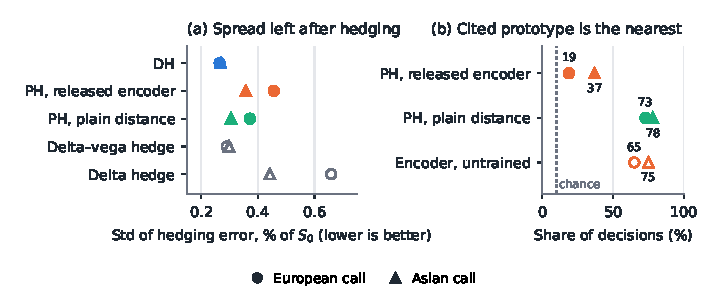
\includegraphics[width=\textwidth]{fig_summary}
\caption{The two results, test period 2022--2024, ten underlyings weighted equally, five seeds averaged.
(a)~Standard deviation of the hedging error in the main setup; the unhedged position has 3.99 (European)
and 2.38 (Asian). (b)~Share of decisions whose highest-weight prototype is also the nearest of its ten
prototypes in the standardised state; hollow markers: the encoder at random initialisation, a reference.}
\label{fig:summary}
\end{figure}

Our contributions are: (i)~\emph{a controlled comparison on historical option data}: ten underlyings,
European and Asian calls, identical inputs, tuning budget and checkpoint rule for both methods, with
specifications frozen before their runs and a single evaluation on 2022--2024; (ii)~\emph{an audit of
prototype explanations on market data}, which separates whether the cited prototypes drive the decision
(they do, for both layers) from whether they resemble the current state (only with plain distance), and
which checks whether prototypes correspond to dated market crises. Fig.~\ref{fig:summary} summarises both.

% ------------------------------------------------------------------------------------------------
\section{ProtoHedge and Related Work}

\paragraph{Learned hedging.} DH parameterises the decision at step $t$ by a network $\pi_\theta(x_t)$ of
the observed state and trains $\theta$ through many price paths to maximise a risk-adjusted utility of
the terminal outcome, typically an optimised certainty equivalent such as CVaR
\cite{rockafellar2000,bental2007oce}. Extensions include no-transaction bands \cite{imaki2021notransaction}, drift
removal \cite{buehler2021drift} and reinforcement learning \cite{halperin2020qlbs,kolm2019dynamic,cao2021deep}.
On historical option data, regressions on standard
sensitivities hedge about as well as neural networks \cite{ruf2022hedging}, and deep hedging has been
trained on historical paths \cite{mikkila2023empirical}. We know
of no evaluation of an interpretable learned hedger on historical option data.

\paragraph{ProtoHedge.} PH keeps DH's objective and replaces the network's output by
\begin{equation}
c(x)=\sum_{k=1}^{K} w_k(x)\,a_k,\qquad w_k(x)=\frac{\exp(-d(x,p_k))}{\sum_{j=1}^{K}\exp(-d(x,p_j))},
\label{eq:proto}
\end{equation}
where $p_1,\dots,p_K$ are the prototypes and $a_k\in[-1,1]^2$ their attached outputs, learned parameters.
The prototypes are fixed before training: a small DH agent is trained, the states it visits are clustered
by $k$-means \cite{macqueen1967}, and each centre is replaced by the nearest visited state, so every
prototype is a real, dated state. The released code uses an encoder distance
$d(x,p)=\lVert f(\tilde x)-f(\tilde p)\rVert^2$, with $f$ a two-layer network on the standardised state
$\tilde x$. The authors' notebooks record an earlier \emph{plain-distance} layer,
$d(x,p)=\sum_j\lambda_j(\tilde x_j-\tilde p_j)^2$ with learned $\lambda_j>0$. We report both; the
released encoder is our main PH model.

\paragraph{Where the decomposition holds.} Equation~(\ref{eq:proto}) is exact for the output $c$. In the
main setup the position is $h_t=\mathrm{clip}\big((\Delta^{\mathrm{liab}}_t,0)+c(x_t)\big)$: the model
delta of the liability in the underlying, plus the correction, then position and trade limits. The
prototypes therefore explain the learned correction to the delta hedge, not the delta itself; the limits
rarely bind (PH positions sat at a limit in 0.12\% of test decisions on average). An attached output $a_k$ is
what the model learned to do near state $p_k$, not a trade anyone made on that date.

\paragraph{Evaluating prototype explanations.} Prototype networks explain by pointing at training cases
\cite{li2018prototypes,chen2019looks,rudin2019stop}. Learned similarity need not match similarity in the
inputs \cite{hoffmann2021looks}, so explanations are best judged by functional tests
\cite{doshivelez2017rigorous,nauta2023anecdotal}: necessity, robustness \cite{alvarezmelis2018robustness}
and comparison with an untrained model \cite{adebayo2018sanity}.

% ------------------------------------------------------------------------------------------------
\section{Data and Backtest}
\label{sec:data}

\paragraph{Task.} Each episode has $T=20$ daily decisions. At the start the hedger is short one synthetic
at-the-money call on the underlying with strike $S_0$: European, paying $\max(S_T-S_0,0)$, or
arithmetic-average Asian, paying $\max(\bar A-S_0,0)$, where $\bar A$ averages the 20 closing prices after
the start \cite{kemna1990asian}. The hedger trades the underlying and one listed call. All prices are
divided by $S_0$. With positions $h_t$ held after trading at $t$, trades $a_t=h_t-h_{t-1}$ ($h_{-1}=0$),
costs $\kappa_t$ per unit and liability payment $H\le0$, the outcome is
\begin{equation}
O=H+\sum_{t=0}^{T-1}h_t^{\top}(P_{t+1}-P_t)-\sum_{t=0}^{T-1}\kappa_t^{\top}\lvert a_t\rvert .
\label{eq:outcome}
\end{equation}
The \emph{hedging error} $E=O+V_0$ adds back the premium $V_0$, the liability's model value at the start,
so a perfect hedge has $E\approx0$.

\paragraph{What is historical and what is modelled.} Historical: closing prices of the underlying (CRSP
\cite{crspStock}), end-of-day quotes of the listed call (OptionMetrics IvyDB \cite{wrdsOptionMetrics}),
traded at the bid--ask midpoint, and that call's implied volatility, delta $\Delta_t$ and vega $\nu_t$ as
supplied by OptionMetrics. Modelled: the liability's value $V_0$ and its delta and vega, from
Black--Scholes \cite{black1973pricing} for the European call and Lévy's lognormal moment matching for the
Asian call (fixings already observed enter through the running average), with zero rates and the listed
call's implied volatility on that day. Decisions use the day's closing data and trade at those prices.
Costs follow the original study: $0.0002\,S_t$ per share and $0.02\,\nu_t+0.0002\,|\Delta_t|+0.0005\,C_t$
per listed call, where $C_t$ is its mid price and $\nu_t$ the price change per unit of volatility; prices
and vega are in units of $S_0$, so a cost of $0.001$ is 0.1\% of the initial price. At the end positions
are marked at the final mid price without a liquidation cost, and the liability is settled at its payoff.
Positions and daily trades are limited to $[-1,1]$ per instrument.

\paragraph{Episodes.} We use AAPL, IWM, NVDA, QQQ, SPY, TLT, XLE, XLF, XLK and XLV over 2005--2024. The
calendar is split first: training to 2018, validation 2019--2021, test 2022--2024, with a 20-day gap at
each boundary. On each start date we choose one listed call with 20--40 days to expiry and strike within
10\% of spot (closest to the money, then to 30 days, then tightest spread) and keep it for the episode. An
episode is kept only if that contract expires after the episode and has a valid quote (positive bid, no
crossed market) on all 21 observation dates with unchanged terms. This eligibility rule looks ahead at
quote availability, though no decision does; it also excludes episodes across stock splits and contract
adjustments (no kept episode has a one-day price move beyond 40\%). This gives 20,537 training, 6,881
validation and 6,977 test episodes. Episodes overlap in 19 of 20 days, so a ticker's roughly 2,000
training episodes hold only about 100 non-overlapping months. A policy observes the
underlying and listed-call prices, the time left, the listed call's implied volatility, log-moneyness and
time to expiry, its two positions and, for the Asian call, the running average.

\paragraph{Rule-based hedges.} The \emph{delta hedge} holds $\Delta^{\mathrm{liab}}_t$ units of the
underlying. The \emph{delta--vega hedge} also neutralises sensitivity to volatility: it holds
$\nu^{\mathrm{liab}}_t/\nu_t$ listed calls and adjusts the share position by their delta. Both use the
same costs and limits as the learned policies.

% ------------------------------------------------------------------------------------------------
\section{Protocol}
\label{sec:protocol}

\paragraph{Three setups.} In each, both methods receive identical inputs, objective, output meaning and
training. (i)~\emph{Original settings}: the output is a trade, the objective CVaR at 50\% of $O$, the state
holds prices, time left and positions, DH has width 20 and PH $K=100$. (ii)~\emph{Equal tuning, original
objective}: the tuned configuration of (iii) trained on CVaR$_{50}(O)$. (iii)~\emph{Main setup}: the output
is the correction to the delta hedge described above and the objective is the variance of $E$. In all
setups inputs are standardised with training statistics and outputs start near zero.

\paragraph{Tuning and training.} Both methods received the same search on validation data of three
development tickers (SPY, TLT, NVDA): three output meanings, three objectives, two state sets and five
sizes per method. Mean validation rank selected $K=10$ for both PH layers and width 128, depth 3, for DH
(tied with width 256; we kept the size closer to the original). These configurations were frozen for all
tickers. Training uses Adam (learning rate $10^{-3}$, batch 32) for at most 2,000 epochs with patience
150, keeping the epoch with the best validation objective. Prototypes come from a width-20 DH agent of the
same ticker, option and seed; each PH layer clusters its own bank. The main setup has five seeds per
ticker and option, the others three. All 1,120 fits passed an integrity check (budget, checkpoint, reload,
independent re-simulation, limits, prototype provenance) and all enter every average.

\paragraph{Measures.} The \emph{original utility} $U=\mathrm{CVaR}_{50}(O)$ is the mean of the worst half
of outcomes, reported as the gain over not hedging, in units of $S_0$ (higher is better). \emph{Spread
removed} is $1-\mathrm{std}(E)/\mathrm{std}(E_{\mathrm{unhedged}})$, the reduction in the standard
deviation of the hedging error. The \emph{worst-5\% loss} CVaR$_5(E)$ is the mean of the worst 5\% of
hedging errors, in \% of $S_0$ (negative; closer to zero is better). Results average seeds within each
ticker, then tickers with equal weight.

\paragraph{Uncertainty and the twelve primary contrasts.} The 6,977 test episodes are not independent:
they overlap in time and the tickers move together. Intervals therefore come from a paired circular block
bootstrap \cite{politis1992} that resamples 20-day blocks of calendar dates and keeps every ticker's
episode on each drawn date (2,000 draws). They capture the sampling variability of test-period market
paths for fixed trained models; averaging five seeds reduces training noise but retraining variability is
not in the intervals. Twelve contrasts were declared primary: PH $-$ DH, DH $-$ delta hedge and PH $-$
delta hedge, on std$(E)$ and CVaR$_5(E)$, for both options, with Holm adjustment \cite{holm1979simple}.
All other intervals are secondary and unadjusted.

\paragraph{History of the evaluation.} The test dates were examined in an earlier version of this study
with different models. The present specifications were frozen before their runs, and the test episodes
were evaluated once. The explanation audit (Sect.~\ref{sec:explain}) was designed after that evaluation;
its pass marks were recorded before it ran, but two were set with the corresponding values already known
(marked $\ddagger$ in Table~\ref{tab:audit}). We treat it as exploratory.

\paragraph{Simulation check.} The authors' code reproduces their simulated result with default seeds
(Table~\ref{tab:original}); in four extra restarts PH stayed within 1.5\% of DH under stochastic volatility,
but failed to train in 2 of 4 Black--Scholes restarts (gaps of $-23\%$, $-30\%$).

\paragraph{Use of AI tools.} An AI assistant (Claude, Anthropic \cite{anthropicClaude2026}) was used to
write and run the experiment and analysis code, to draft the pre-declared protocols, and to draft and edit
this manuscript; an earlier version of the data pipeline was written with OpenAI Codex
\cite{openaiCodex2026}. The authors directed the study, reviewed protocols, code, results and text, and are
responsible for the content.

% ------------------------------------------------------------------------------------------------
\section{Q1: How Much Hedging Performance Does ProtoHedge Retain?}
\label{sec:results}

\begin{table}[t]
\caption{The original paper's comparison. Gain over not hedging in the utility $U=\mathrm{CVaR}_{50}(O)$,
in units of $S_0$ (higher is better); PH minus DH with 95\% interval; $|U_{\mathrm{DH}}|$, DH's utility
level; Rel.\ = (PH $-$ DH)$/|U_{\mathrm{DH}}|$, the original paper's convention (the paper rows quote its
published values, which do not give $U_{\mathrm{DH}}$); spread removed. BS/SV: simulated Black--Scholes and stochastic-volatility markets; ``rerun'': authors' code and
default seeds. Equal tuning and Main: setups (ii) and (iii); encoder/plain: the two PH layers. Historical: test 2022--2024, tickers equal-weighted, seeds averaged. Intervals are secondary
contrasts without multiplicity adjustment; $^{\dagger}$computed after the main evaluation.}
\label{tab:original}
\centering
\scriptsize
\setlength{\tabcolsep}{0.9pt}
\begin{tabular}{@{}>{\raggedright\arraybackslash}lrrlrrr@{}}
\toprule
Setting & DH gain & PH gain & PH $-$ DH [95\% interval] & $|U_{\mathrm{DH}}|$ & Rel. & Removed \\
 & & & & & & DH/PH, \% \\
\midrule
\multicolumn{7}{@{}l}{\emph{Simulated markets (authors' code and 5,000-path test set)}} \\
\quad BS, paper & +0.04570 & +0.04547 & $-$0.00023 & -- & $-$0.40\% & -- \\
\quad BS, rerun & +0.04566 & +0.04549 & $-$0.00020 & 0.05821 & $-$0.34\% & -- \\
\quad SV, paper & +0.03440 & +0.03410 & $-$0.00030 & -- & $-$0.33\% & -- \\
\quad SV, rerun & +0.03438 & +0.03417 & $-$0.00021 & 0.09024 & $-$0.23\% & -- \\
\midrule
\multicolumn{7}{@{}l}{\emph{Historical data, European call (delta hedge: gain +0.02766, 83\% removed)}} \\
\quad Original settings & +0.02114 & +0.02122 & +0.00008 [$-$0.00665, +0.00737] & 0.04059 & +0.2\% & 29 / 20 \\
\quad Equal tuning & +0.03056 & +0.02919 & $-$0.00137 [$-$0.00366, +0.00140] & 0.03118 & $-$4.4\% & 28 / 41 \\
\quad Main, encoder & +0.02570 & +0.02625 & +0.00056 [+0.00000, +0.00106]$^{\dagger}$ & 0.03603 & +1.5\% & 93 / 89 \\
\quad Main, plain & +0.02570 & +0.02437 & $-$0.00133 [$-$0.00187, $-$0.00080] & 0.03603 & $-$3.7\% & 93 / 91 \\
\midrule
\multicolumn{7}{@{}l}{\emph{Historical data, Asian call (delta hedge: gain +0.01537, 81\% removed)}} \\
\quad Original settings & +0.00944 & +0.00989 & +0.00045 [$-$0.00385, +0.00523] & 0.02695 & +1.7\% & $-$14 / $-$14 \\
\quad Equal tuning & +0.01591 & +0.01478 & $-$0.00112 [$-$0.00394, +0.00212] & 0.02048 & $-$5.5\% & $-$15 / 13 \\
\quad Main, encoder & +0.01278 & +0.01343 & +0.00065 [+0.00041, +0.00086]$^{\dagger}$ & 0.02361 & +2.7\% & 89 / 85 \\
\quad Main, plain & +0.01278 & +0.01298 & +0.00020 [$-$0.00005, +0.00042] & 0.02361 & +0.9\% & 89 / 87 \\
\bottomrule
\end{tabular}

\end{table}

\paragraph{On the original utility.} Table~\ref{tab:original} repeats the original comparison on
historical data. The released encoder is not detectably behind DH in any setup: its gaps lie between
$-5.5\%$ and $+2.7\%$ of DH's utility, and in the main setup it is ahead, detectably for the Asian call
(interval computed after the evaluation). The plain-distance layer is detectably behind DH for the European
call ($-0.00133$, $[-0.00187,-0.00080]$). Intervals containing zero do not show equivalence: up to forty
times wider than in simulation, they cannot confirm the half-percent margin seen there.

\paragraph{The utility does not measure hedging.} Under the original settings, DH and PH remove only 29\%
and 20\% of the European call's error spread and \emph{increase} the Asian call's by 14\%; 54 of 120 fits
end with more spread than not hedging, and both gain less utility than the delta hedge. The objective
explains most of this: CVaR at 50\% of an outcome that excludes the premium is weakly risk-averse, so on
drifting prices a directional position can score like a hedge \cite{buehler2021drift}. With that objective
even the tuned policies of setup (ii) remove at most 41\%, whereas the main setup removes 85--93\%.

\begin{table}[t]
\caption{Hedging quality in the main setup, test 2022--2024. Removed: reduction in std$(E)$ relative to
not hedging. Std $E$, worst-5\% loss CVaR$_5(E)$ (closer to zero is better) and mean trading cost in \% of
$S_0$. The rows above the line are rule-based hedges.}
\label{tab:hedging}
\centering
\scriptsize
\setlength{\tabcolsep}{3.4pt}
\begin{tabular}{@{}lrrrrcrrrr@{}}
\toprule
 & \multicolumn{4}{c}{European call} && \multicolumn{4}{c}{Asian call} \\
\cmidrule{2-5}\cmidrule{7-10}
Strategy & Removed & Std $E$ & CVaR$_{5}$ & Cost && Removed & Std $E$ & CVaR$_{5}$ & Cost \\
\midrule
Unhedged & 0.0\% & 3.99 & $-$10.75 & 0.00 && 0.0\% & 2.38 & $-$6.38 & 0.00 \\
Delta hedge & 83.5\% & 0.66 & $-$1.48 & 0.04 && 81.4\% & 0.44 & $-$1.13 & 0.03 \\
Delta--vega hedge & 92.7\% & 0.29 & $-$1.09 & 0.39 && 87.4\% & 0.30 & $-$1.07 & 0.30 \\
\midrule
DH & 93.3\% & 0.27 & $-$0.84 & 0.31 && 88.7\% & 0.27 & $-$1.00 & 0.38 \\
PH, released encoder & 88.5\% & 0.46 & $-$1.27 & 0.25 && 84.9\% & 0.36 & $-$1.17 & 0.32 \\
PH, plain distance & 90.7\% & 0.37 & $-$1.21 & 0.36 && 87.2\% & 0.31 & $-$1.05 & 0.30 \\
\bottomrule
\end{tabular}

\end{table}

\paragraph{Hedging quality.} Table~\ref{tab:hedging} gives the main setup. PH removes 88.5\% and 84.9\% of
the spread, DH 93.3\% and 88.7\%. A gap of four percentage points in spread removed is a large relative
gap in what remains: PH's error spread is 1.72 (European) and 1.33 (Asian) times DH's. PH's spread is
wider than DH's in all ten tickers (Fig.~\ref{fig:tickers}) and its worst-5\% loss is larger (primary
contrasts, PH $-$ DH in \% of $S_0$: std$(E)$ $+0.19$ $[0.16,0.21]$ and $+0.09$ $[0.07,0.11]$;
CVaR$_5(E)$ $-0.43$ $[-0.51,-0.31]$ and $-0.16$ $[-0.25,-0.07]$; Holm $p=0.006$ for all four). Both learned
methods narrow the spread relative to the delta hedge (primary, $p=0.006$); on the worst-5\% loss only
the European comparisons are detectable. The strong classical comparator is the delta--vega hedge, which
removes 92.7\% and 87.4\%: more than PH on both options (secondary: $+0.17$ $[0.14,0.19]$ and $+0.06$
$[0.03,0.09]$), slightly less than DH. PH thus does not dominate simple hedges: it beats the delta--vega
hedge on the original utility but not on spread. The plain-distance layer sits between PH and DH (90.7\%
and 87.2\%; 1.40 and 1.14 times DH's spread). PH also trades less than DH (Table~\ref{tab:hedging}), which may contribute to its small utility lead.

\begin{figure}[t]
\centering
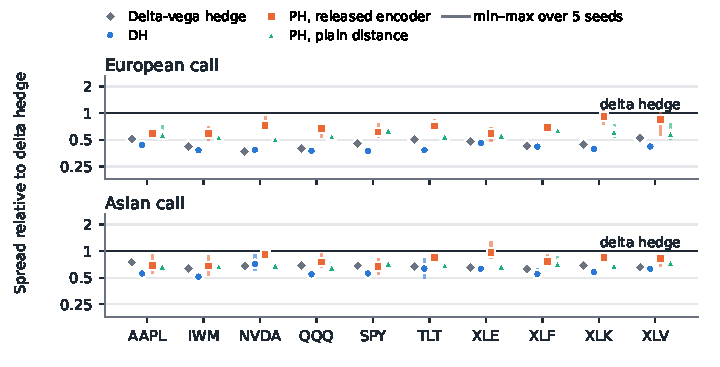
\includegraphics[width=\textwidth]{fig_tickers}
\caption{Robustness by ticker: spread of the hedging error relative to the delta hedge (horizontal line;
log scale, lower is better), main setup, test 2022--2024. Markers: mean over five seeds; vertical bars:
min--max across the five training seeds.}
\label{fig:tickers}
\end{figure}

\paragraph{Training data.} The gap shrinks with more data. On validation data of the development
tickers, PH's spread relative to the delta hedge falls from 0.93 and 1.03 with a quarter of a ticker's
history to 0.51 and 0.64 with all of it (DH: 0.42/0.65 to 0.27/0.44), and one model trained on all ten
tickers removes 92.2\% and 88.8\% on the test period (DH 94.0\% and 90.7\%). This is suggestive, not a
controlled test.

% ------------------------------------------------------------------------------------------------
\section{Q2: When Can a Reader Trust the Cited Prototype?}
\label{sec:explain}

\begin{table}[!t]
\caption{Explanation audit, main setup, test 2022--2024, 100 fits per layer (10 tickers, 2 options, 5
seeds), equal-ticker means. \textsc{p}/\textsc{f}: meets or misses the pass mark recorded before the run.
$^{\ddagger}$Pass mark set with the value already known. Nearest: Euclidean distance in the standardised
state (market features, time features and the two positions) among the fit's ten prototypes, unweighted
for both layers. Recall: pass requires a rise with block-bootstrap interval above zero. Sufficiency also
requires a top-3 output error of at most 0.10 output sd. Fallback acts on decisions farther from every prototype, in the market
features, than 95\% of training decisions.}
\label{tab:audit}
\centering
\scriptsize
\setlength{\tabcolsep}{1.6pt}
\begin{tabular}{@{}>{\raggedright\arraybackslash}p{1.6cm}>{\raggedright\arraybackslash}p{3.45cm}>{\raggedright\arraybackslash}p{0.8cm}cccc@{}}
\toprule
 & & & \multicolumn{2}{c}{Released encoder} & \multicolumn{2}{c}{Plain distance} \\
\cmidrule(lr){4-5}\cmidrule(l){6-7}
Test & Measure & Pass mark & European & Asian & European & Asian \\
\midrule
\multicolumn{7}{@{}l}{\emph{Influence}} \\
Stability & Heaviest prototype unchanged under 0.1 sd noise & $\ge$90\% & 94\% \textsc{p} & 91\% \textsc{p} & 92\% \textsc{p} & 94\% \textsc{p} \\
Local removal & Output change, 3 heaviest / 3 lightest removed (sd) & $\ge$3$\times$, $\le$0.05 & 0.63/0.00 \textsc{p} & 0.76/0.00 \textsc{p} & 0.35/0.01 \textsc{p} & 0.75/0.01 \textsc{p} \\
Deletion & Corr.\ of use with std$(E)$ rise on deletion & $\ge$0.5 & 0.69 \textsc{p} & 0.73 \textsc{p} & 0.46 \textsc{f} & 0.52 \textsc{p} \\
\midrule
\multicolumn{7}{@{}l}{\emph{Visible similarity}} \\
Nearest$^{\ddagger}$ & Heaviest is nearest of 10 (chance 10\%) & $\ge$50\% & 19\% \textsc{f} & 37\% \textsc{f} & 73\% \textsc{p} & 78\% \textsc{p} \\
\midrule
\multicolumn{7}{@{}l}{\emph{Crisis correspondence}} \\
Represent. & Prototypes in stress windows (9.4\% of days) & $\ge$14\% & 20\% \textsc{p} & 24\% \textsc{p} & 22\% \textsc{p} & 23\% \textsc{p} \\
Recall & Their weight, calm $\to$ stressed test days & rise & 17$\to$20\% \textsc{p} & 20$\to$26\% \textsc{p} & 13$\to$26\% \textsc{p} & 15$\to$28\% \textsc{p} \\
\midrule
\multicolumn{7}{@{}l}{\emph{Reading and use}} \\
Sufficiency$^{\ddagger}$ & std$(E)$ change, top 3 prototypes only & $\le$5\% & 7\% \textsc{f} & 15\% \textsc{f} & 63\% \textsc{f} & 35\% \textsc{f} \\
Self-consist. & Output at own state vs attached output (sd) & $\le$10\% & 14\% \textsc{f} & 23\% \textsc{f} & 18\% \textsc{f} & 28\% \textsc{f} \\
Fallback & std$(E)$ change, delta hedge far from bank & $<$0 & +15\% \textsc{f} & +12\% \textsc{f} & +23\% \textsc{f} & +11\% \textsc{f} \\
\bottomrule
\end{tabular}

\end{table}

\paragraph{Tests.} An explanation is a decision's prototype weights, the dated prototypes and their
attached outputs. Table~\ref{tab:audit} groups the tests by question. \emph{Influence}: is the decision
stable under noise smaller than a typical daily move (0.1 vs.\ a median of 0.14--0.20 sd), does removing
the three heaviest prototypes change it while removing the three lightest does not, and does deleting a
prototype from the whole hedge raise std$(E)$ in proportion to its use? \emph{Visible similarity}: is
the cited prototype also the nearest one in the state a reader sees? \emph{Crisis correspondence} uses
six stress windows of 2008--2018 fixed from the public record (2008--09, 2010, 2011,
2015, two in 2018), and calls a test day stressed if its implied volatility is in the top 10\%.

\paragraph{Influence holds; visible similarity depends on the layer.} For both layers the explanations are
stable and the cited prototypes matter: removing the three heaviest changes the output by 0.35 to 0.76
standard deviations, removing the three lightest by at most 0.01. Deleting a prototype hurts the hedge in
proportion to its use, except narrowly for the plain European call (correlation 0.46, mark 0.5). Influence
is not similarity, however. With plain distance the heaviest prototype is the nearest one in 73\% and 78\%
of decisions; with the released encoder in 19\% and 37\%, against 10\% by chance. The untrained encoder
scores 65\% and 75\%, so training moves the encoder's notion of similarity away from the visible features,
as reported for image models \cite{hoffmann2021looks}. A plain-distance explanation is a weighted distance
on named features, with most weight on the listed call's log-moneyness (41\% and 32\%) and then on the
positions held. Three negative results hold for both layers: the three heaviest prototypes alone do not
reconstruct the hedge (the spread changes by 7--63\%); the output at a prototype's own state differs from
its attached output by 14--28\% of an output standard deviation; and falling back to the delta hedge far
from every prototype widens the spread by 11--23\%.

\paragraph{Crises.} Prototypes are disproportionately crisis days: 20\% to 24\% come from the stress
windows, which hold 9.4\% of training days. On stressed test days the weight on them rises, clearly for
plain distance (13\% to 26\%, 15\% to 28\%) and modestly for the encoder (17\% to 20\%, 20\% to 26\%);
named 2022--2024 events give the same result. (A test on the largest trades failed, but those
mostly open an episode.)

\begin{figure}[t]
\centering
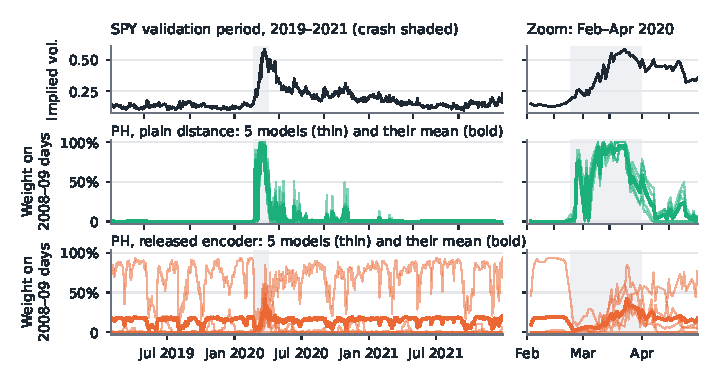
\includegraphics[width=\textwidth]{fig_covid}
\caption{SPY European calls, selected validation case (2019--2021, not used for training; chosen after
the audit). Top: median implied volatility of the listed calls. Below: daily mean weight on prototypes
dated in the 2008--09 crisis, for the five plain-distance and five encoder models (seeds 0--4; within a
seed both layers share the data and the DH agent that supplies their prototypes, but cluster their own
banks). Right: February--April 2020. Shaded: 24 February to 31 March 2020.}
\label{fig:covid}
\end{figure}

\paragraph{What a dated explanation lets a reader inspect: March 2020.} Fig.~\ref{fig:covid} follows the
SPY models through the validation years (used for their stopping epochs). In calm 2019 the five plain-distance models put under 0.2\% of their weight on
2008--09 days. In the COVID crash (24 February to 31 March 2020) they put 49\% to 71\% there. Three cite
29 September 2008 as their heaviest prototype, the day the S\&P~500 fell 8.8\% after the US House rejected
the bank rescue; its attached
output roughly keeps the delta hedge and adds about a third of a listed call. The other two cite the
first week of March 2009. During the crash these models held 0.37 to 0.55 listed calls, close to that
attached output, where the delta hedge would hold none. The encoder models differ from one another: three
raise their crisis weight from near zero to 11--26\% in the crash, one never uses crisis prototypes, and
one weights them at 68\% in 2019 and 21\% in the crash, so their mean barely moves. Over the 20 hedges
open on 16 March 2020 the mean absolute hedging error was 1.5\% of $S_0$ for plain distance, 1.1\% for the
encoder, 0.5\% for DH, 2.7\% for the delta hedge and 3.6\% unhedged. This shows which days the models weighted,
not that they understood either crisis.

% ------------------------------------------------------------------------------------------------
\section{Conclusion}

On historical option data ProtoHedge keeps most of Deep Hedging's risk reduction but not all of it: it
removes 88.5\% and 84.9\% of the hedging-error spread against 93.3\% and 88.7\%, leaving 1.7 and 1.3 times
DH's spread, and it trails a delta--vega hedge. On the original utility the released model is not behind
DH in our comparisons, which shows how little that utility says about hedging. Its explanations are
influential and stable, but only the plain-distance layer cites prototypes that usually resemble the
current state. In this study plain distance makes retrieval auditable at a moderate cost in spread, DH gives
the narrowest errors, and the March 2020 example shows what a dated explanation lets a reader inspect.

\paragraph{Limitations.} Liabilities are synthetic, costs stylised, trades execute at the closing mid quote, and eligibility
requires a complete future quote path; we study ten US underlyings and one maturity range. The test period
had been examined before, intervals omit retraining variability, the audit is functional and exploratory,
and the March 2020 case was selected afterwards. Two of 100 encoder fits and 13 of 100 plain-distance fits
reached the epoch limit.

\paragraph{Data and code.} OptionMetrics and CRSP data are licensed through WRDS and cannot be
redistributed. Code, configurations and the pre-declared protocols are available from the authors on
request.

\bibliographystyle{splncs04}
\bibliography{references}

\end{document}
